\documentclass[11pts]{amsbook}
\usepackage{../HBSuerDemir}
\begin{document}
\hPage{198}
\section{\underline{CYLINDRICAL AND SPHERICAL COORDINATE SYSTEMS}}
\subsection{\underline{CylindIrical coordinate systems (Polar coordinate systems in 3-space).}}
\begin{minipage}{0.55\textwidth}

\qquad A rectangular coordinate system Oxyz in which xy-plane is taken as polar plane (with x-axis as polar axis) is called a
\underline{cylindrical coordinate system}.

\qquad Cylindrical coordinates of a
point P are $\Theta$, r,z and one writes $P(\Theta, r, z).$

\qquad When the coordinates of a point P are given, plotting of
P is done in the order $\Theta$,r and z, while having a point P its coordinates are obtained in the order z, r, $\Theta$.

\end{minipage}
\begin{minipage}{0.45\textwidth}
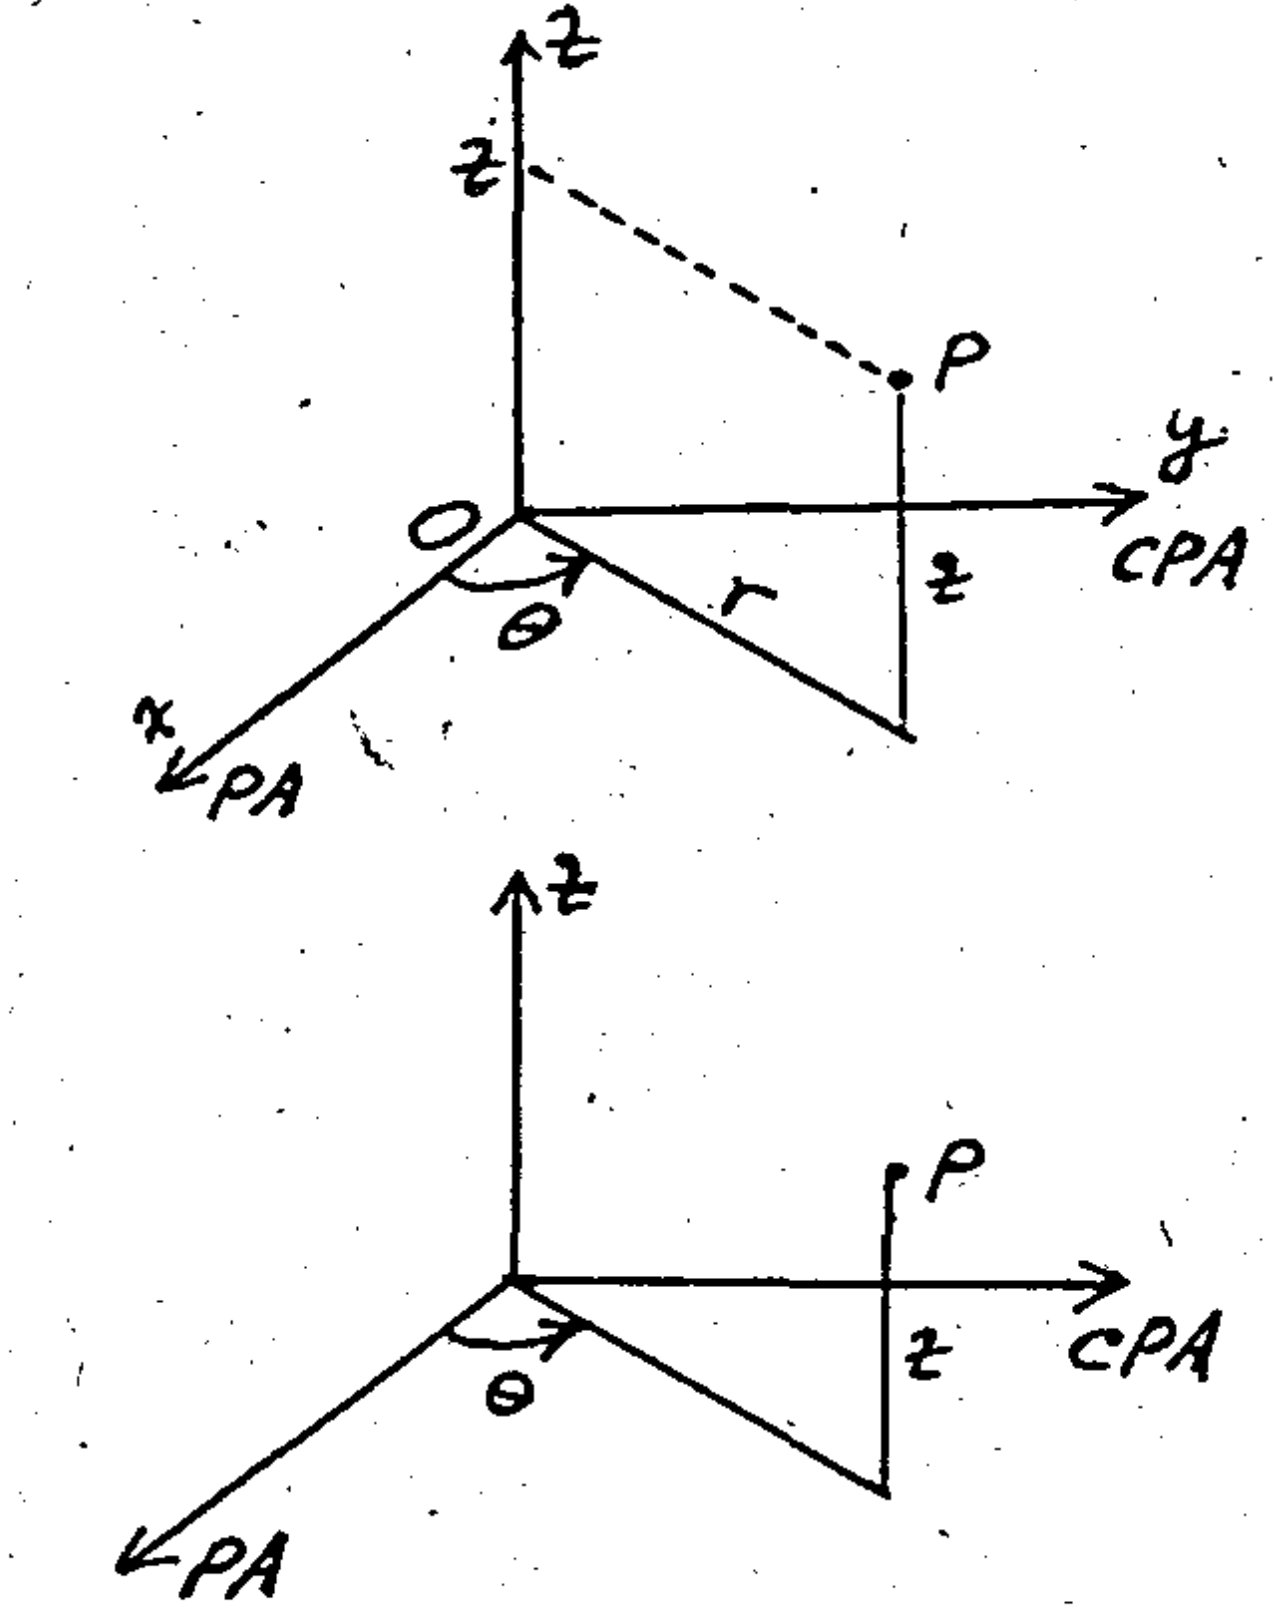
\includegraphics[width=\textwidth]{images/b2p1-198-fig01}
\end{minipage}

\qquad \underline{Transforming relations.}
% in the original text cylindrical was written as cylildrical, so I have corrected it.

\qquad These are the relation between cartesian coordinates
X, y, Z and cylindrical ones $\Theta$, r, Z of an arbitrary point P:

\qquad x = r cos$\Theta$\qquad \qquad \qquad $\Theta$ =  arctan $\frac{y}{x}$

\qquad y =  r  sin$\Theta$\qquad or \qquad r =  $ \pm \sqrt{x^2+y^2}$

\qquad z = z \qquad \qquad \qquad z = z

\qquad $\Theta$-constant surfaces are planes through z-axis surfaces are circular right cylinders with Oz as axis, and z-constant surfaces are horizontal planes.






\end{document}
